\section{コンポーネントAPIの設計}

アプリケーション内でコンポーネントを特定する場合、そのコンポーネントがどのような目的を持ち、他のコンポーネントからどのように使用されるかを考えることから始める必要があります。代表的なコンポーネントには、情報管理、プロセッサ、ファサードなどがあります。情報マネージャーは、メモリ内または外部のデータストアにある状態を追跡し、データの作成、変更、問い合わせの操作を提供します。プロセッサーは、データの変換や計算を行うコンポーネントである。ファサードコンポーネントは、主に別の外部システムにアクセスできるようにする(プラグイン可能な)ために存在します。

実際には、ほとんどのコンポーネントはこれらの箱にきれいに収まるわけではなく、1つまたは複数の側面を組み合わせて、独自のアプリケーションのユニークなニーズを満たすコンポーネントにします。

コンポーネントを設計する際に最初に考慮すべきことは、外部の消費者が使用するAPIです。コンポーネントとの対話には、主に2つの方法があります。関数を呼び出す方法と、キューやチャネルでメッセージを渡す方法です。まず、関数について見てみましょう。

\subsection{関数によるコンポーネントデータの操作}

API関数は、外部の消費者がコンポーネントと対話できるようにするための、ノブ、ボタン、またはゲージのようなものです。Clojureでは、多くのものがユーザーによって関数として呼び出されますが、関数、マクロ、プロトコル、マルチメソッドなど、異なる実装があります。(他のもの-マップ、セット、キーワード、シンボルなど-はAPIの一部としてあまり有用ではありません)。

コンポーネントレベルに焦点を合わせましたが、これまで学習したことをすべて覚えておく必要があります。可能な限り、コンポーネントはイミュータブルなデータを直接公開すべきです。イミュータブルであるため、コンポーネントのデータの一部をコンシューマーに渡しても害はありません:コピーは必要ありませんし、コンポーネント自身のデータが影響を受けることもありません。呼び出し元がデータを手に入れたら、自由にClojureツールを使ってクエリや変換を行うことができます。

リクエストを受け取り、自動応答を形成するために使用されるルールのセットを管理する知識エンジンのコンポーネントを考えてみましょう。ルールの具体的なフォーマットはひとまず置いておいて、各ルールがデータとして定義されていると仮定します。ルールを追加、置換、削除するためのAPI関数と、何らかの基準に基づいてルールを検索するための関数が必要です。また、ルールを起動し、手元の作業を行うための関数も必要である。

\begin{lstlisting}[numbers=none]
;; 注:keはステートフル知識エンジン・コンポーネントを指す
;; Read interface
(defn get-rules [ke])
(defn find-rules [ke criteria])
;; Update interface
(defn add-rule [ke rule])
(defn replace-rule [ke old-rule new-rule])
(defn delete-rule [ke rule])
;; Processing interface
(defn fire-rules [ke request])
\end{lstlisting}

そして、これらの関数を次のように使うことができる。

\begin{lstlisting}[numbers=none]
(defn example [] (let [ke (new-ke)]
    (add-rule ke :r1)
    (add-rule ke :r2)
    (add-rule ke :r3)
    (replace-rule ke :r1 :r1b)
    (delete-rule ke :r3)
    (get-rules ke)))
\end{lstlisting}

しかし、もう少し深く見てみると、より小さな関数の集合でAPI全体をサポートできることがわかります。

\begin{lstlisting}[numbers=none]
;; Get the rule-set
(defn get-rules [ke])
;; Transform from one rule-set to another
(defn transform-rules [ke update-fn])
;; Produce a response from a request
(defn fire-rules [ke request])
\end{lstlisting}

\texttt{find-rules}関数は\texttt{get-rules}に対するフィルタリングとして実装することができる.\texttt{add-rule}、\texttt{replace-rule}、\texttt{delete-rule}関数はすべて、ルールセット全体に対する\texttt{transform-rules}の適用と見なすことができる。

ほとんどのAPIはこのパターンを持っている。つまり、少数の重要な基本関数と、使いやすさのために提供されるより大きな関数群である。プロトコルは、複数の実装がそのプロトコルを拡張できるように、機能の中核となるセットを捕捉する良い方法である。派生機能はAPIネームスペースで提供され、プロトコルの上にレイヤー化されるべきである。API関数は、プロトコルを拡張するあらゆるエンティティで動作する。

これを完全な名前空間にまとめると、次のようになる。

\begin{lstlisting}[numbers=none]
(ns components.ke)

;; SPI protocol
(defprotocol KE
  (get-rules [ke] "Get full rule set")
  (transform-rules [ke update-fn]
    "Apply transformation function to rule set. Return new KE.")
  (fire-rules [ke request]
    "Fire the rules against the request and return a response"))

;; private helper functions
(defn- transform-criteria [criteria]
  ;; ...
  )

;; api fns built over the protocol
(defn find-rules
  [ke criteria]
  (filter (transform-criteria criteria) (get-rules ke)))

(defn add-rule
  [ke rule]
  (transform-rules ke #(conj % rule)))

(defn replace-rule
  [ke old-rule new-rule]
  (transform-rules ke #(-> % (disj old-rule) (conj new-rule))))

(defn delete-rule
  [ke rule]
  (transform-rules ke #(-> % (disj rule))))
\end{lstlisting}

この実装では、図にあるように、小さな拡張可能な抽象化(サービスプロバイダインタフェース)の上にコンポーネントAPIを重ねる形で定義しています。

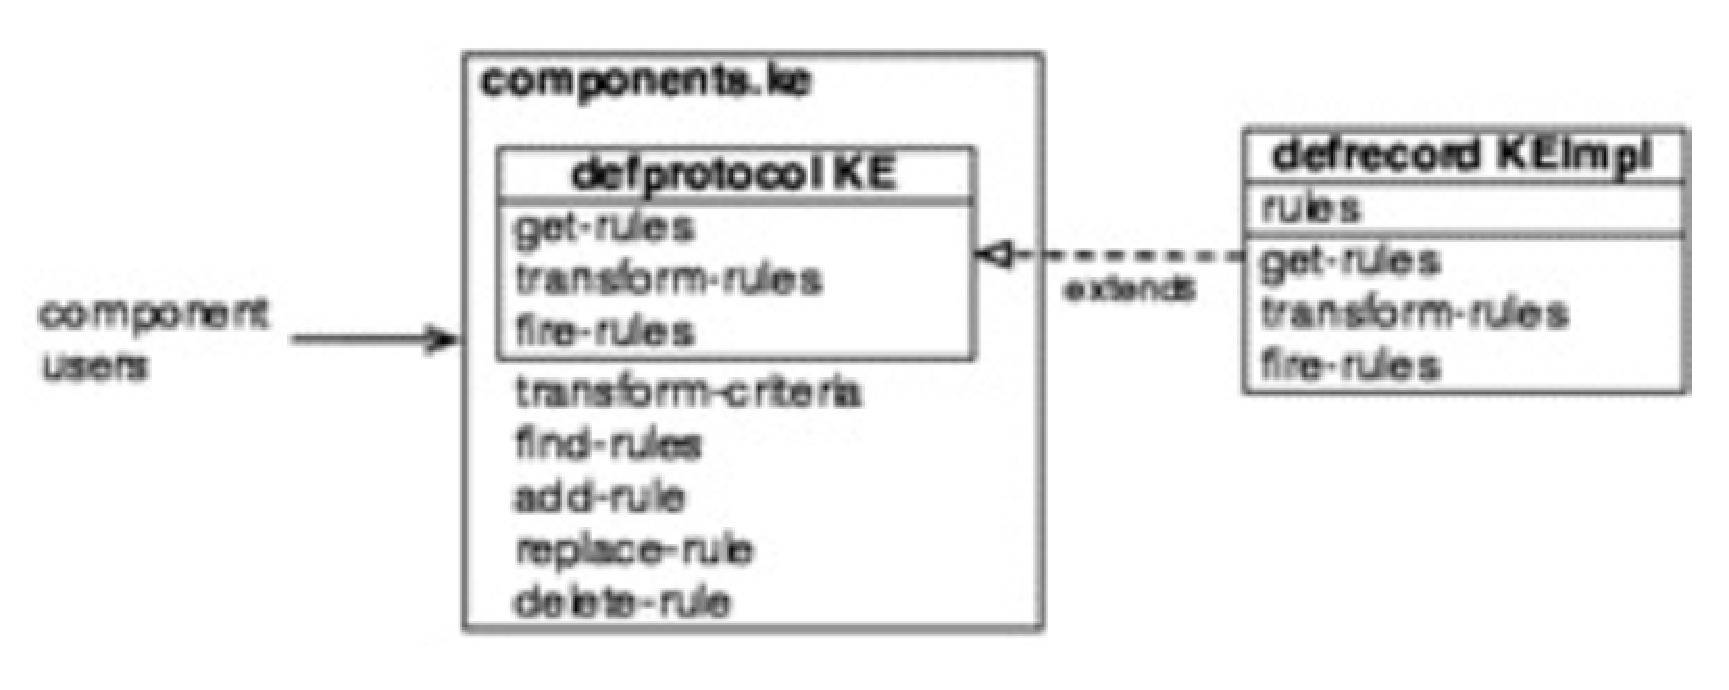
\includegraphics[width=10cm]{fig_06_002.eps}

API全体のプロトコルを作成すると、どのような実装でもすべての関数を再実装する必要があります。その代わり、Clojureで関連する関数のセットを収集するための最適なツールは、プロトコルではなく名前空間です。プロトコルは、今回のように拡張のための最小限の抽象化を定義しているときに最適です。

このコンポーネントの状態実装部分については後で説明し、今は非同期呼び出しなど、他のAPIに関する考察に焦点を合わせます。


\subsection{非同期API}

第5章「コアを使う」では、非同期API関数に対して1回限りの非同期応答を提供するためのfuturesやpromiseといったツールについて既に説明しました。前のセクションで出てきた \texttt{fire-rules} 関数を考えてみましょう。レスポンスを生成するのに時間がかかるかもしれないので、呼び出し元をブロックするのではなく、futureを返すこともできます。

\begin{lstlisting}[numbers=none]
  (let [response-future (fire-rules ke request)]
    ;; ... other work...
    @response-future) ;; レスポンスを取得するために参照する
\end{lstlisting}

応答のためにブロックするのではなく、futureを返すことで、呼び出し側がブロックするタイミングを選択できる(futureをdereferencingすることで)。もう一つの選択肢は、ここに示すように、コールバックを受け取るか(関数を呼び出す)、プロミスを返すか(結果を提供する)である。


\begin{lstlisting}[numbers=none]
;; 知識エンジンが起動するfire-rulesにコールバックを送る。
(let [callback (fn [response] ...)]
  (fire-rules ke request callback))

  ;; 知識エンジンが応答を返すために使うpromiseを送る
(let [result-promise (fire-rules ke request)]
  ;; 必要なときにresult-promiseを参照する。
  @result-promise)
\end{lstlisting}

非同期API呼び出しにどちらが適しているかは、APIそのものよりも呼び出し側のコードに依存します。

さて、直接または非同期の関数呼び出しでAPIを作成する方法を見てきましたが、アプリケーションの寿命を通じてより永続的な関係でコンポーネントを接続する方法についても検討する必要があります。






